\documentclass[9pt]{beamer}
\usetheme{Madrid}
\usepackage[utf8]{inputenc}
\usepackage{amsmath}
\usepackage{amsfonts}
\usepackage{amssymb}
\usepackage{physics}

\setbeamerfont{alerted text}{series=\bfseries}
\setbeamerfont{structure}{series=\bfseries}
\setbeamerfont{title}{series=\bfseries}
\setbeamerfont{subtitle}{series=\bfseries}
\setbeamerfont{frametitle}{series=\bfseries}

\usepackage[style=verbose,bibencoding=utf8,backend=bibtex]{biblatex}
%\addbibresource{/home/matthew/masters_articles/references.bib}
% \addbibresource{/home/matthew/github/masters_presentation/references.bib}
\addbibresource{references.bib}
\setbeamerfont{footnote}{size=\tiny}
%\renewcommand*{\thefootnote}{[\arabic{footnote}]}

\AtBeginBibliography{\small}
\setbeamertemplate{bibliography item}{}

\setbeamertemplate{navigation symbols}{}

\setbeamercolor{author in head/foot}{bg=white}
\setbeamercolor{title in head/foot}{bg=white}
\setbeamercolor{date in head/foot}{bg=white}
\setbeamercolor{date in head/foot}{fg=white}


\begin{document}

% \title[U-net automated contouring]{Clinical implementation of deep learning:
  \title[]{Clinical implementation of deep learning:

	Automatic contouring via  U-Net architecture}

% \author[Matthew Cooper]{\textbf{Matthew Cooper}\inst{1}\\ \small{Simon Biggs\inst{2}\\ Yu Sun\inst{1}\\ Matthew Sobolewski\inst{2}}}
\author[]{\textbf{Matthew Cooper}\inst{1}\\ \small{Simon Biggs\inst{2}\\ Yu Sun\inst{1}\\ Matthew Sobolewski\inst{2}}}

\date[]{}

% \institute[USyd]{\inst{1} The University of Sydney (USyd). School of Physics.
 \institute[]{\inst{1} The University of Sydney (USyd). School of Physics.

	Institute of Medical Physics.
	\vspace{2mm}

	\inst{2} Riverina Cancer Care Centre (RCCC). Cancer Care Associates.
	\vspace{6mm}

	\small \textbf{Thesis:} \href{https://github.com/matthewdeancooper/masters_thesis}{github.com/matthewdeancooper/masters\_thesis}
	\vspace{1mm}

	\textbf{Video overview:} \href{https://docs.pymedphys.com/background/autocontouring.html}{docs.pymedphys/com/background/autocontouring}
	\vspace{7mm}

	\noindent
	\hspace{-0.25cm}
	\begin{minipage}[b]{\textwidth}
    	\centering
    	\raisebox{-0.5\height}{
\includegraphics[height=1.0cm, keepaspectratio]{images/usyd}}
    	\hspace*{3mm}
    	\raisebox{-0.5\height}{
\includegraphics[height=0.7cm, keepaspectratio]{images/rcc}}
    	\hspace*{2mm}
    	\raisebox{-0.5\height}{
\includegraphics[height=1.6cm, keepaspectratio]{images/pymedphys_title}}
  	\end{minipage}
  }


% ---------------------------- DOCUMENT ---------------------------------

\maketitle




%\begin{frame}{Introduction: Contouring}
%\begin{columns}
%\column{0.5\textwidth}
%\begin{itemize}
%	\item Contouring defines and classifies volumes within the patient.
%	\item Allows for a mapping of beam output to anatomy.
%	\item Calculate dose distribution to a volume within patient for a treatment plan.
%
%	ie. Dose volume histogram (DVH):
%\end{itemize}
%
%\column{0.5\textwidth}
%\begin{figure}
%	\includegraphics[width=\textwidth]{images/contour}
%	\caption{Single posterior field setup for carbon ion treatment of pancreatic cancer. Multiple contours present.\footnotemark[1]}
%\end{figure}
%\end{columns}
%\footnotetext[1]{\fullcite{Dreher2017}}
%\end{frame}

% ---------------------------- FRAME ---------------------------------
\begin{frame}{Contouring - Current limitations }
\textbf{Variability}
\begin{itemize}
\item Large intra and inter-observer variance (IOV).\footnotemark[1]
\item  AAPM TG275 risk assessment - multiple human-factor failure modes in RT.\footnotemark[2]
	%Mean surface distance (MSD), Dice coefficient (DSC)
	%\begin{itemize}
	%	\item Bladder: MSD 0.99(0.30) mm, DSC 0.93 $\pm$ 0.03
	%	\item Rectum: MSD 2.862(2.066) mm, DSC 0.81 $\pm$ 0.07
	%\end{itemize}
\end{itemize}
\footnotetext[1]{\fullcite{Roach_2019}}
\footnotetext[2]{\fullcite{Ford2020}}
\vspace{4mm}

\textbf{Time constraints}
\begin{itemize}
	% \item Manual $\implies$  $\leq$ 4 hrs (head \& neck).\footnotemark[3]
	\item Atlas methods $\implies$ significant correction times.\footnotemark[3]
	\item Barrier to future technologies that require fast contouring.\footnotemark[3]
	% \begin{itemize}
	% 	\item Adaptive RT
	% \end{itemize}
\end{itemize}
\vspace{4mm}

\textbf{Deep learning potential}
\begin{itemize}
	\item Shown to reduce IOV and contouring time.\footnotemark[3]
	\item Significant improvement cf. atlas methods (time \& accuracy).\footnotemark[4]
	% \item Poor performance on class imbalanced data (local minima trapping).\footnotemark[5]
	% \item Fail to generalise to independent site data.\footnotemark[5]
\end{itemize}
\footnotetext[3]{\fullcite{Vinod_2016}}
\footnotetext[4]{\fullcite{Nikolov_2018}}
% \footnotetext[5]{\fullcite{Hesamian2019}}
\end{frame}
%

% ---------------------------- FRAME ---------------------------------
\begin{frame}{Research goals}

% \textbf{Model 1:} QA tool (RCCC) - Pelvic imaging (Patient, bladder, rectum).
\textbf{Model 1:} QA tool - Pelvic imaging for prostate cancer.
\begin{itemize}
%\item Manual contouring.
% \item Potential to manage some prominent hazards identified by the task group TG275
\item Contour patient, bladder, rectum volumes
\item Alert if prediction differs significantly from expert.
\item Need for delineation to be part of regular QA.\footnotemark[4]

\end{itemize}
\vspace{4mm}

% \textbf{Model 2:} Automatic contouring (SASH) - Canine vacuum bag
\textbf{Model 2:} Automatic contouring - Canine vacuum bag
\begin{itemize}
\item Automate time consuming aspect of canine RT
\item Previously, manual vacuum bag contouring $\approx$ 30 min
% \item Lower barrier to entry wrt. implementation.
\end{itemize}
\vspace{3mm}

\textbf{Goal:} Performance similar to human experts.
\begin{itemize}
\item Performance metric (sDSC) that takes into account expert IOV.\footnotemark[3]
% \item Stronger correlation with correction time cf. DSC.\footnotemark[5]
  % \item Generalise model performance to independent patient data.
\end{itemize}
\footnotetext[3]{\fullcite{Nikolov_2018}}
\footnotetext[4]{\fullcite{Vinod_2016}}
% \footnotetext[5]{\fullcite{Vaassen_2020}}
\end{frame}

% ---------------------------- FRAME ---------------------------------

\begin{frame}{Performance - Surface dice similarity coefficient (sDSC)}
  \begin{equation*}
    DSC_{1,2} = \frac{2|M_{1} \cap M_{2}|}{|M_{1}| + |M_{2}|}
    \label{eq:sDSC}
  \end{equation*}

  \vspace{4mm}

  \begin{equation*}
    sDSC_{1,2}^{(\tau)} = \frac{|S_{1} \cap B_{2}^{(\tau)}| + |S_{2} \cap B_{1}^{(\tau)}|}{|S_{1}| + |S_{2}|}
    \label{eq:sDSC}
  \end{equation*}

  \vspace{4mm}
  \begin{figure}
    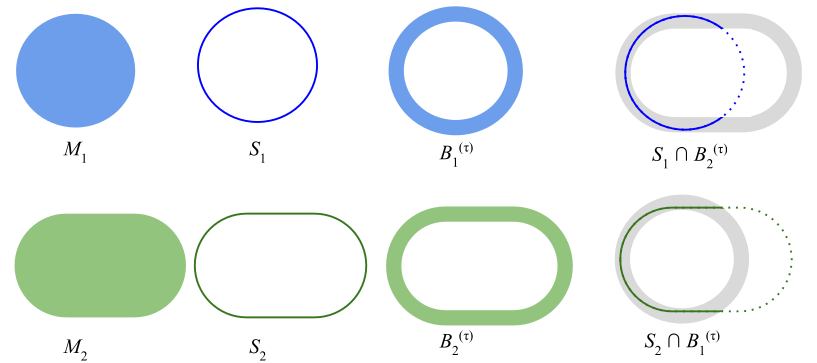
\includegraphics[width=0.6\textwidth]{images/sDSC}
    % \caption{Clinical performance metric: Illustration of volume masks $M_{i}$, surfaces $S_{i}$, boundaries $B_{i}^{(\tau)}$ at organ specific tolerance $\tau$, and intersection of surface boundaries $S_{i} \cap B_{j}^{(\tau)}$. Value states the percentage of surface contoured within expert IOV.\footnotemark[3]}
  \end{figure}
  \footnotetext[3]{\fullcite{Nikolov_2018}}
\end{frame}

% ---------------------------- FRAME ---------------------------------
%
% ---------------------------- FRAME ---------------------------------
% \section{Theory}
% \begin{frame}{Theory: Machine learning}
% %\textbf{Machine learning}
% \begin{itemize}
% 	\item Iterative process of improving (training) a map \textbf{$f$}: $Input$ $\to$ $Output$
% 	\item Performance defined by some loss function $\sim$ $\norm{f(Input) - Output}$
% 	\item 'Learning' $\implies$ $\downarrow$ loss
% 	\item \textbf{Aim}: Learning generalises to new data
% \end{itemize}
% \begin{figure}
% 	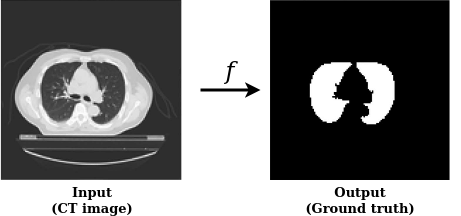
\includegraphics[width=0.6\textwidth]{images/model_input_output_2}
% 	\caption{Generalised map from a model input (CT image) to the ground truth (Expert segmentation mask).\footnotemark[6]}
% \end{figure}
% \footnotetext[6]{\fullcite{Nemoto_2020}}
% \end{frame}


% ---------------------------- FRAME ---------------------------------
\vspace{4mm}
% \begin{frame}{Theory: Deep learning}
% %\textbf{Deep learning}
% \begin{itemize}
% %\item Machine learning with neural nets (NN) as the architecture %for \textbf{$f$}
% \item Layers of operators with trainable parameters (Feature extraction)
% \begin{itemize}
% 	\item Convolution
% \end{itemize}
% \item Non-trainable parameters
% \begin{itemize}
% 	\item Pooling layers (Feature selection)
% 	\item Non-linear activation functions (ReLU \& Softmax)
% 	\item Regularisation constraints (Dropout \& BatchNorm)
% \end{itemize}
% \item Stochastic gradient descent (SDG) updates parameters to minimise loss.
% \end{itemize}
% \begin{figure}
% 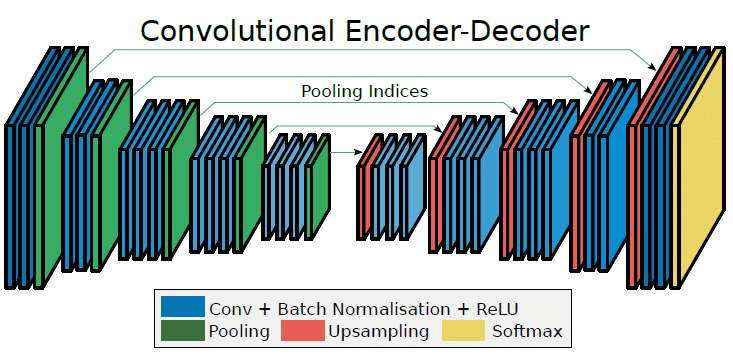
\includegraphics[width=0.5\textwidth]{images/FCNN}
% \caption{5 layer 2D U-net architecture. MaxPooling layers preform down-sampling in the encoder path.\footnotemark[7]}
% \end{figure}
% \footnotetext[7]{\fullcite{Ghosh2018}}
% \end{frame}
%

% ---------------------------- FRAME ---------------------------------
% \section{Method}
% \begin{frame}{Method: Data examination}
% \begin{itemize}
% \item Significant data cleaning required for consistency.
% \item Data split at patient level - training, validation and test independence.\footnotemark[3]
% \item Significant class imbalance
% \end{itemize}\
% \begin{table}[h]
\footnotesize
\caption{Data distribution for pelvic imaging.}
\centering
\begin{tabular}{c c c c c}
\hline\hline
& Training & Validation & Testing & Total  \\ [0.5ex]
\hline

Images(Patients) & 1751(12) & 282(2) & 138(1) & 1991(15) \\
 \\
 \hline\hline
		 & Images total (\%) & Pixel-image ratio (\%)& Pixel-output ratio (\%) & Pixels total (\%)\\ [0.5ex]
\hline
Patient  & 100 & 15.6  &  5.21 & 5.21\\
Bladder  & 28.0 & 0.862 & 0.287 & 0.081\\
Rectum   & 37.0 & 0.172 & 0.057 & 0.021\\
\hline\hline
\end{tabular}
\label{table:data_prostate}
\end{table}

% \begin{table}[h]
\footnotesize
\caption{Data distribution for canine imaging.}
\centering
\begin{tabular}{c c c c c}
\hline\hline
& Training & Validation & Testing & Total  \\ [0.5ex]
\hline

Images(Patients) & 1912(21) & 340(3) & 187(2) & 2439(26) \\
 \\
 \hline\hline
		 & Images total (\%) & Pixel-image ratio (\%)& Pixel-output ratio (\%) & Pixels total (\%)\\ [0.5ex]
\hline
Vacbag   & 70.0& 13.4  & 13.4  &  9.4 \\

\hline\hline
\end{tabular}
\label{table:data_vet}
\end{table}

% \footnotetext[3]{\fullcite{Nikolov_2018}}
% \end{frame}

% ---------------------------- FRAME ---------------------------------
% \begin{frame}{Method: Data augmentation}
% \begin{itemize}
% \item Small datasets a common challenge in medical imaging.\footnotemark[8]
% \item \textbf{Augmentation:} Increase effective dataset size


% ie. $\uparrow$ training data variance $\implies$ $\uparrow$ model robustness.\footnotemark[4]$^{,}$\footnotemark[9]
% \begin{itemize}
% \item L/R image flip
% \item Random crop and resize
% \item Elastic \& affine deformations
% \item Gaussian noise
% \end{itemize}
% %
% \item \textbf{Input normalisation}
% \begin{itemize}
% \item Reduces skew in loss topology $\implies$ accelerate gradient descent (learning).\footnotemark[10]
% \end{itemize}
% \end{itemize}


% \footnotetext[3]{\fullcite{Nikolov_2018}}
% \footnotetext[8]{\fullcite{Ronneberger_2015}}
% \footnotetext[9]{\fullcite{Maier2019}}
% \footnotetext[10]{\fullcite{zhou2018normalization}}
% \end{frame}

% ---------------------------- FRAME ---------------------------------
% \begin{frame}{}
% \begin{figure}
% 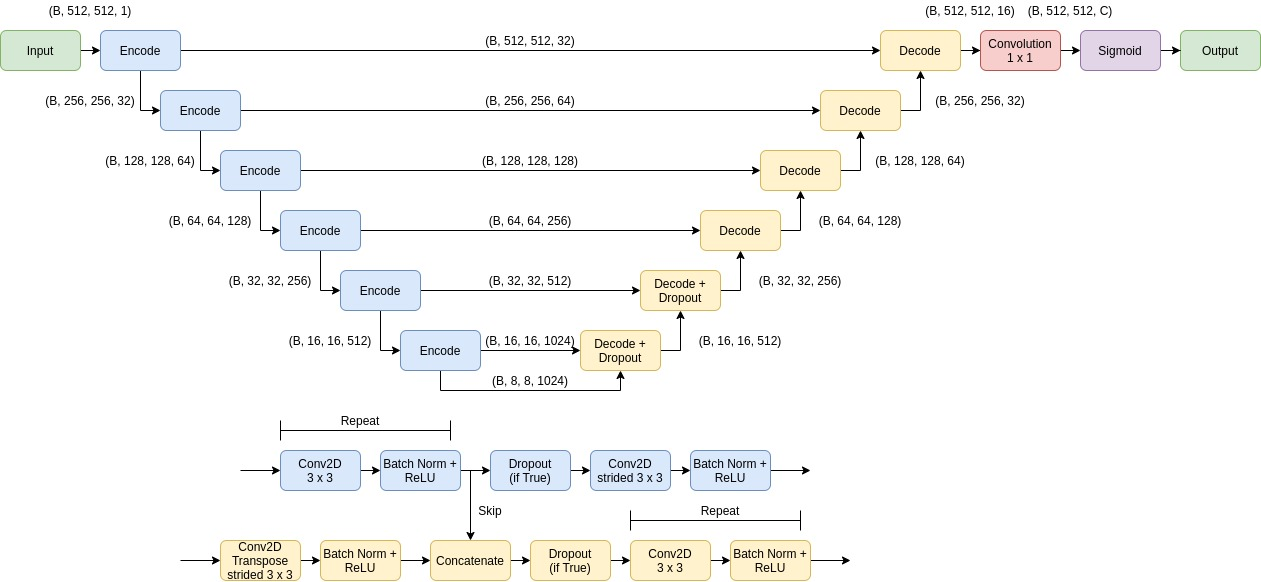
\includegraphics[width=1.0\textwidth]{images/model_diagram}
% \caption{Modified 2D U-net architecture:\footnotemark[8] Composed of encoding (blue) and decoding blocks (yellow). MaxPooling layers replaced by strided convolution.\footnotemark[11] Added batch normalisation\footnotemark[12] and final sigmoid activation.\footnotemark[3] Tensor dimensions (Batch size, X, Y, Channels).}
% \end{figure}
% \footnotetext[3]{\fullcite{Nikolov_2018}}
% \footnotetext[8]{\fullcite{Ronneberger_2015}}
% \footnotetext[11]{\fullcite{springenberg2014}}
% \footnotetext[12]{\fullcite{ioffe2015batch}}
% \end{frame}

%% ---------------------------- FRAME ---------------------------------

% \begin{frame}{Method: Why downsample?}
% \begin{figure}
% 	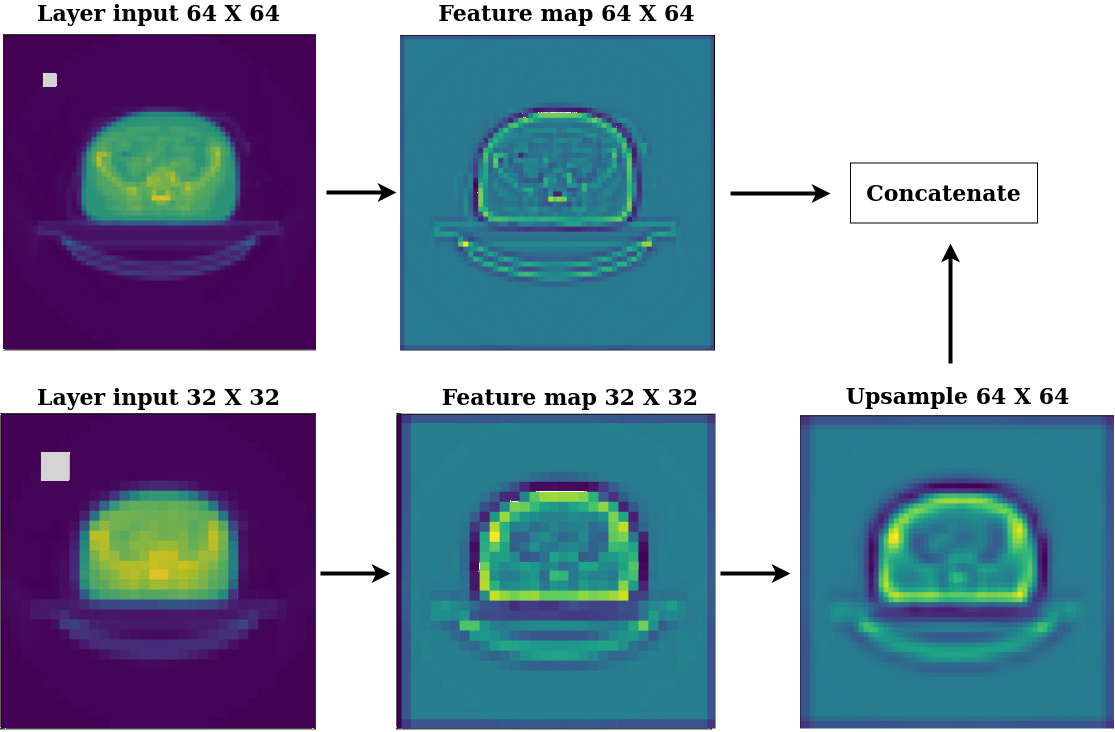
\includegraphics[width=0.75\textwidth]{images/downsampling}
% 	\caption{Multi-resolution analysis: Edge detection shown over encoder-decoder pathway: $\downarrow$ resolution $\implies$ $\uparrow$ relative kernel size (grey) to extract coarser (high level) image features for general localisation. Concatenate with high resolution features for local border segmentation.\footnotemark[6]}
% \end{figure}
% \footnotetext[6]{\fullcite{Nemoto_2020}}
% \end{frame}
%
%
%\begin{frame}{Method: Model hyper-parameters}
%\textbf{Pelvic imaging specific}
%\begin{itemize}
%\item Batch size: 1
%\end{itemize}
%
%\textbf{Canine imaging specific}
%\begin{itemize}
%\item Batch size: 3
%\end{itemize}
%
%\textbf{General}
%\begin{itemize}
%\item Loss: BinaryCrossEntropy (BCE), soft DSC, weighted soft DSC, Focal Tversky.
%\item Optimiser: Adam (Adaptive momentum estimation).\footnotemark[13]
%\item Epochs: Determined by valid loss plateau (20 epoch patience).
%\item Initial learning rate (LR): 1e-5.
%
%
%LR decay x0.5 triggered by valid loss plateau (3 epoch patience)
%\item Initial weights determined by Gaussian distribution.\footnotemark[8]
%
%($\mu=0$, $\sigma=\sqrt{2/in_{weight}}$)
%
%\item Initial convergence via BCE (3 epochs).\footnotemark[14]
%\footnotetext[8]{\fullcite{Ronneberger_2015}}
%\footnotetext[13]{\fullcite{kingma2014}}
%\footnotetext[14]{\fullcite{Bertels2019}}
%\end{itemize}
%\end{frame}

% ---------------------------- FRAME ---------------------------------
%%
\begin{frame}{Modules - All happy models are alike...}
\begin{figure}
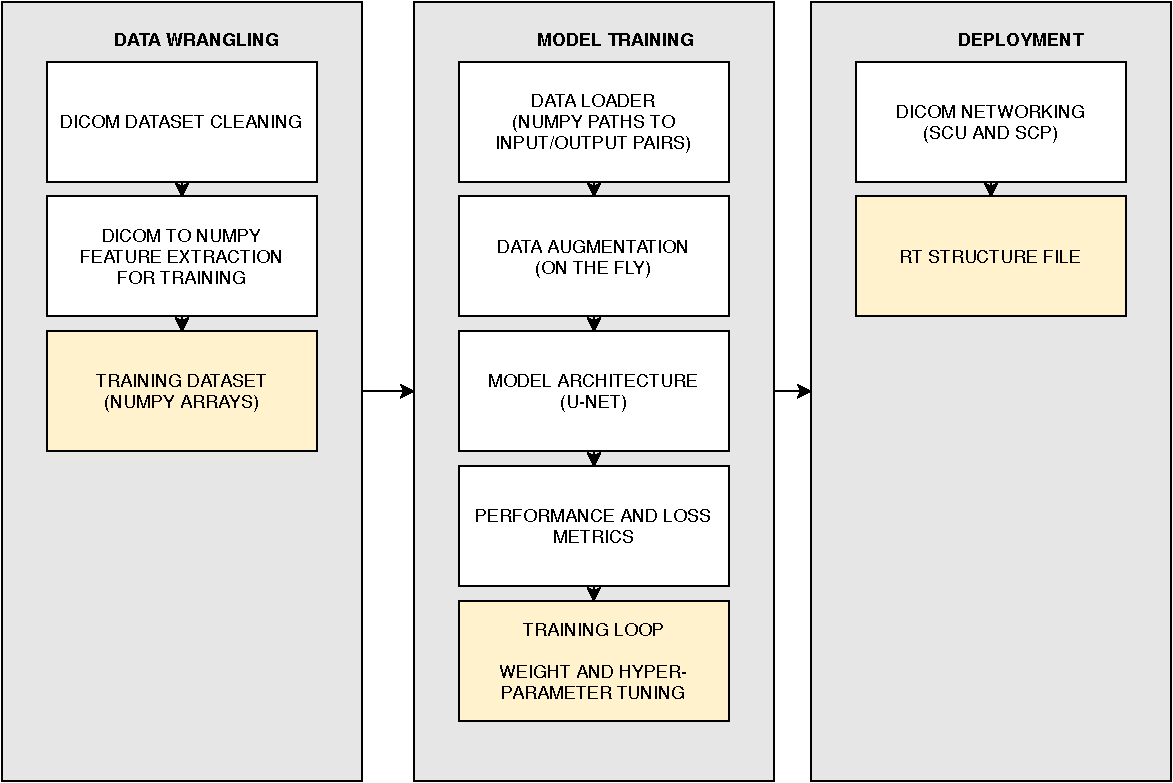
\includegraphics[width=0.85\textwidth]{images/modules}
% \caption{Modules required for end-to-end deep learning model deployment}
\end{figure}
\end{frame}


% ---------------------------- FRAME ---------------------------------
%%
\begin{frame}{Deployment - DICOM networking}
\begin{figure}
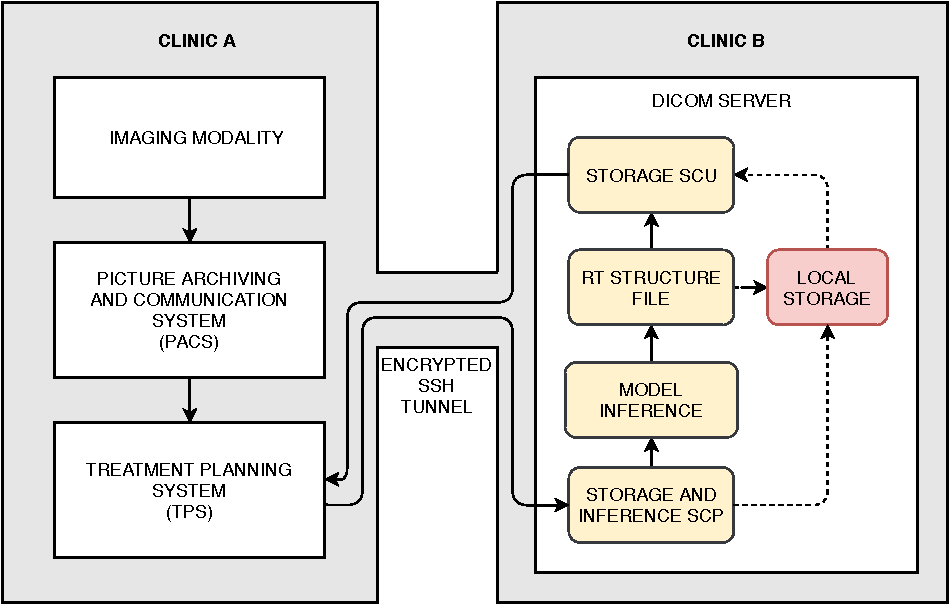
\includegraphics[width=0.75\textwidth]{images/dicom_networking}
% \caption{TPS exports to remote server via DICOM networking protocol}
\end{figure}
\end{frame}
%

% ---------------------------- FRAME ---------------------------------
% \begin{frame}{Method: Forced multi-threading}
%   \begin{figure}
%     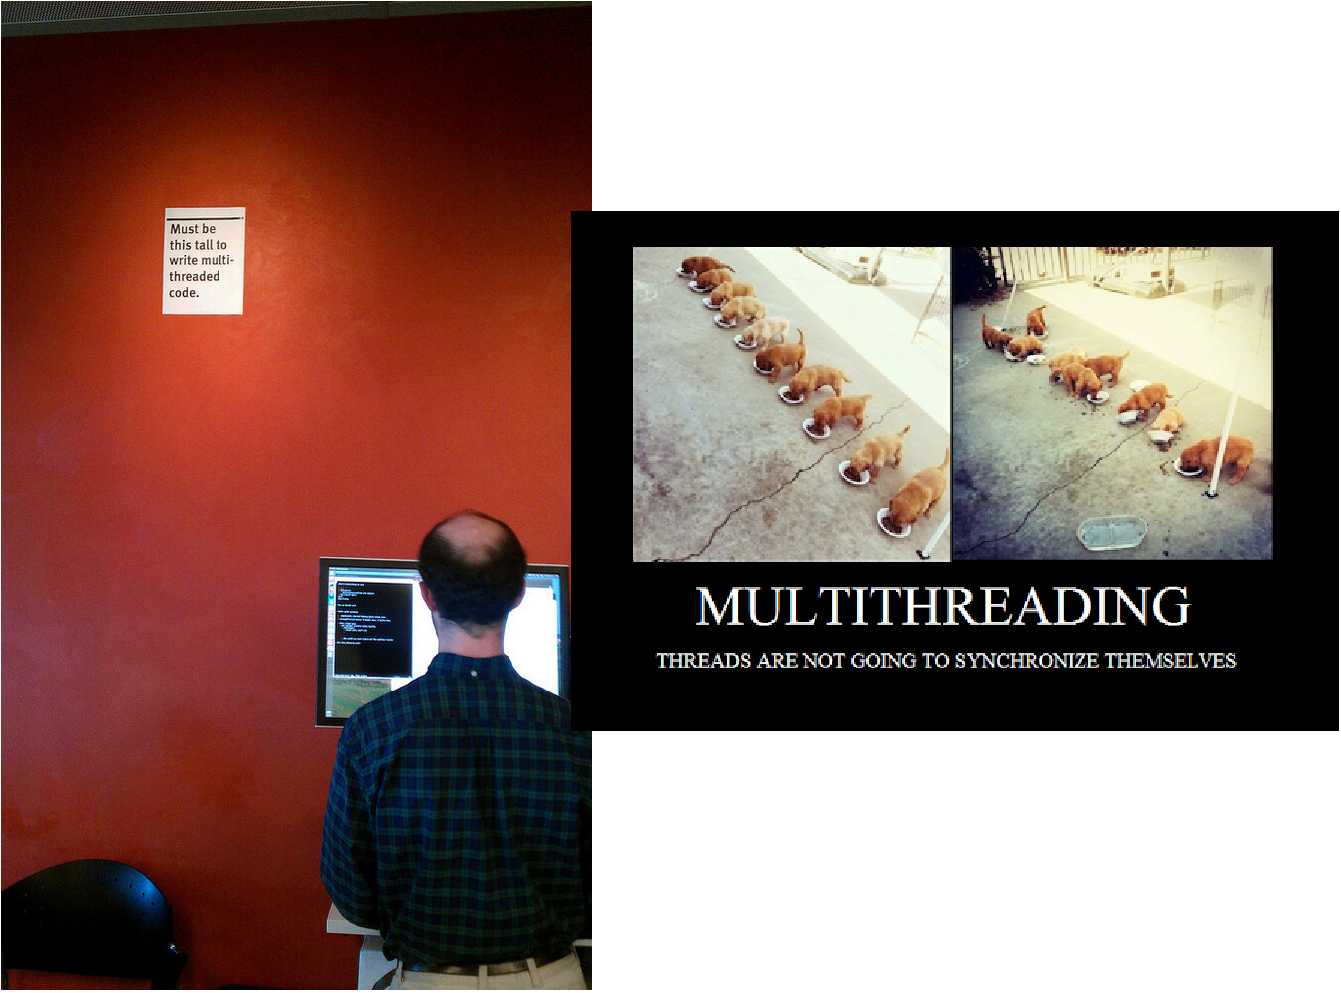
\includegraphics[width=0.99\textwidth]{images/multi}
%     \caption{Pynetdicom forces multi-threaded network associations}
%   \end{figure}
% \end{frame}

% ---------------------------- FRAME ---------------------------------

\section{Results}
% \begin{frame}{Results: Model 1 - metrics for pelvic imaging}
% \begin{table}[h]
\footnotesize
\caption{Loss evaluation on independent test dataset for pelvic imaging}
% title of Table
\centering
% used for centering table
\begin{tabular}{c c c c}
% centered columns (4 columns)
\hline\hline
%inserts double horizontal lines
Loss & DSC & Precision & Sensitivity \\ [0.5ex]
% inserts table
%heading
\hline
% inserts single horizontal line
BinaryCrossentropy (BCE) & 0.995 & 0.999 & 0.991 \\
soft DSC & 0.986 & 0.999 & 0.972 \\
\textbf{w. soft DSC} & \textbf{0.994} & \textbf{0.997} & \textbf{0.991} \\
BCE + 2(w. soft DSC) & 0.985 & 0.999 & 0.971 \\
FocalTversky & 0.962 & 0.941 & 0.987 \\
% [1ex] adds vertical space
\hline\hline
%inserts single line
\end{tabular}
\label{table:loss_prostate}
% is used to refer this table in the text
\end{table}

% \begin{figure}
% 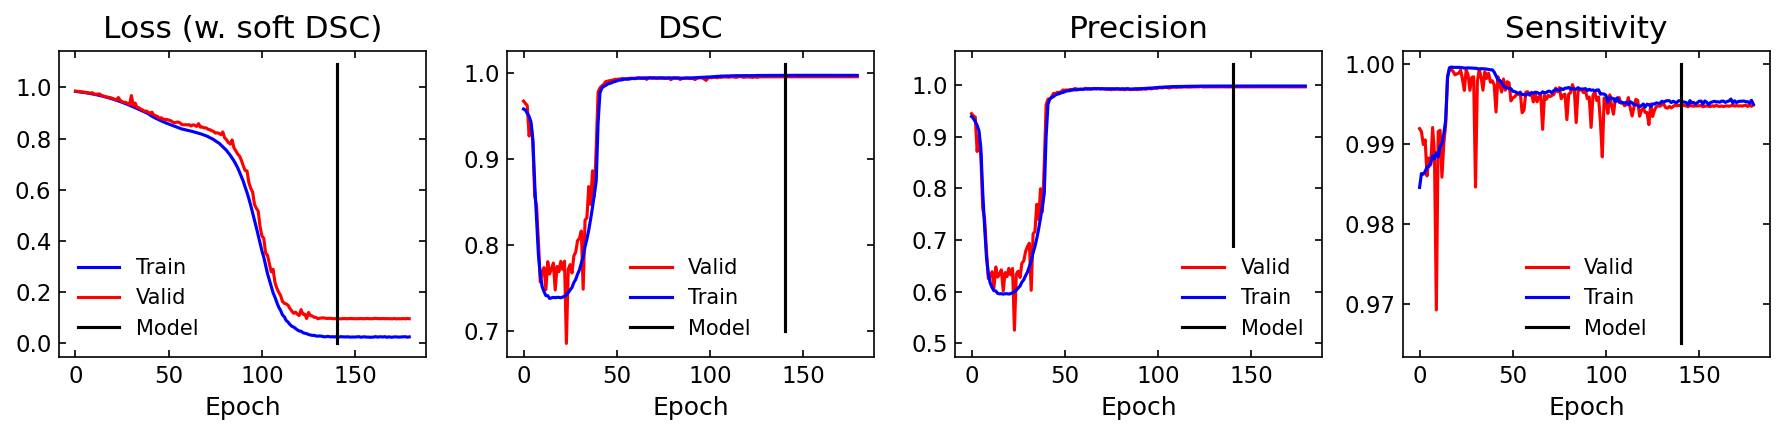
\includegraphics[width=\textwidth]{images/prostate_metrics}
% \caption{Model training metrics for pelvic imaging via weighted soft DSC loss. \textbf{Final model selected at epoch 140} due to validation loss plateau. Metrics begin post BCE weight initialisation (3 epochs). Training time of 9 hours.}
% \end{figure}
% \begin{itemize}
% 	\item \textbf{Inference time:} 3 seconds per patient
% \end{itemize}
% \end{frame}
%
% ---------------------------- FRAME ---------------------------------

%%
\begin{frame}{Pelvic imaging - Patient}
  \begin{figure}
    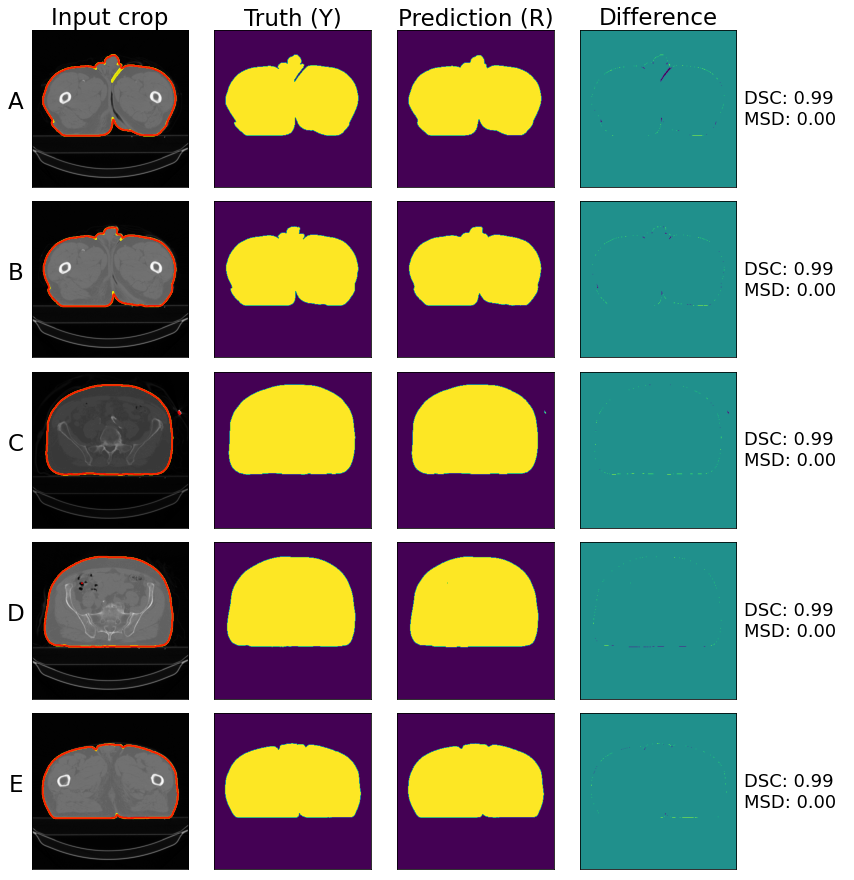
\includegraphics[width=0.65\textwidth]{images/prostate_patient}
    % \caption{Representative output for \textbf{patient}. Truth contour (yellow), prediction contour (red). Mean surface distance (MSD) mm.}
  \end{figure}
\end{frame}
%
% ---------------------------- FRAME ---------------------------------
\begin{frame}{Pelvic imaging - Bladder}
  \begin{figure}
    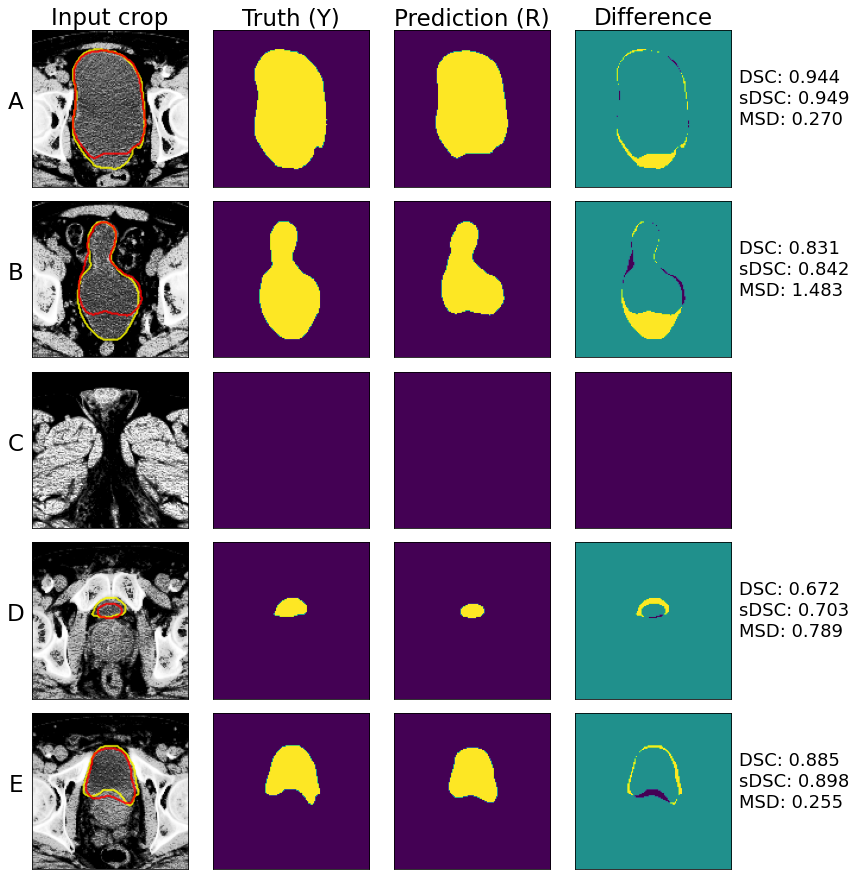
\includegraphics[width=0.65\textwidth]{images/prostate_bladder}
    % \caption{Representative output for \textbf{bladder}. Truth contour (yellow), prediction contour (red). Mean surface distance (MSD) mm. sDSC calculated at $\tau$ of 1.46 mm.}
  \end{figure}
\end{frame}
%
% ---------------------------- FRAME ---------------------------------
\begin{frame}{Pelvic imaging - Rectum}
  \begin{figure}
    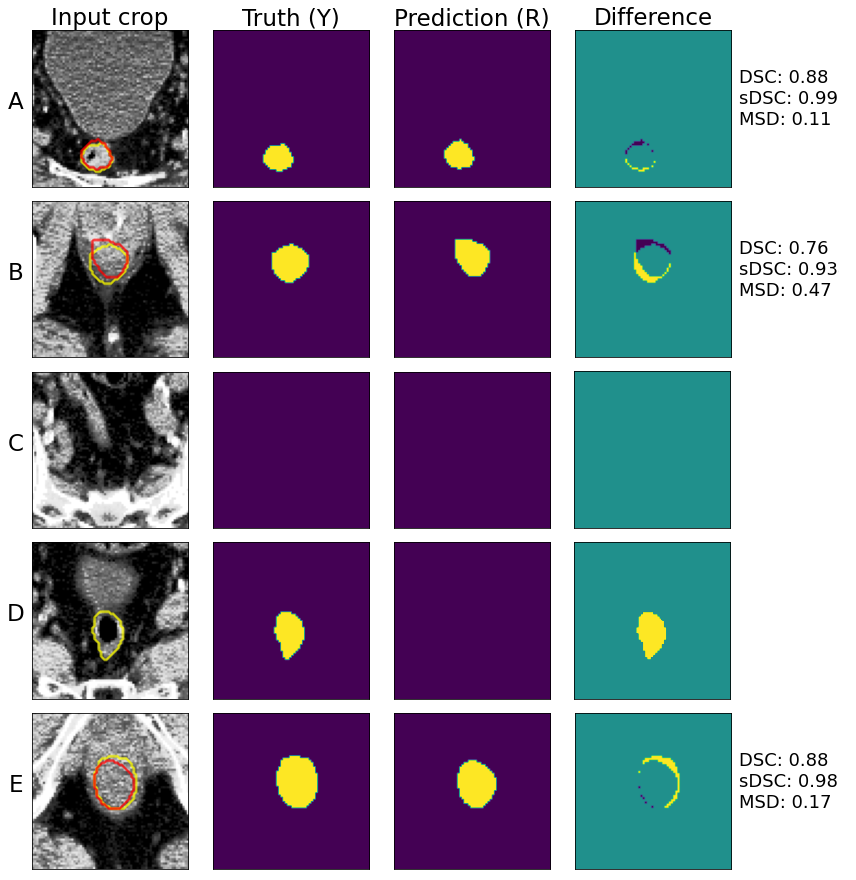
\includegraphics[width=0.65\textwidth]{images/prostate_rectum}
    % \caption{Representative output for \textbf{rectum}. Truth contour (yellow), prediction contour (red). Mean surface distance (MSD) mm. sDSC calculated at $\tau$ of 6.99 mm.}
  \end{figure}
\end{frame}
%
% ---------------------------- FRAME ---------------------------------
% \begin{frame}{Results: Model 2 - metrics for canine imaging}
%   \begin{table}[h]
\footnotesize
\caption{Loss evaluation on independent test dataset for canine imaging}
% title of Table
\centering
% used for centering table
\begin{tabular}{c c c c}
% centered columns (4 columns)
\hline\hline
%inserts double horizontal lines
Loss & DSC & Precision & Sensitivity \\ [0.5ex]
% inserts table
%heading
\hline
% inserts single horizontal line
BinaryCrossentropy & 0.901 & 0.935 & 0.954 \\
\textbf{soft DSC} & \textbf{0.952} & \textbf{0.953} & \textbf{0.953} \\
FocalTversky & 0.930 & 0.906 & 0.969 \\
% [1ex] adds vertical space
\hline\hline
%inserts single line
\end{tabular}
\label{table:loss_vet}
% is used to refer this table in the text
\end{table}

%   \begin{figure}
%     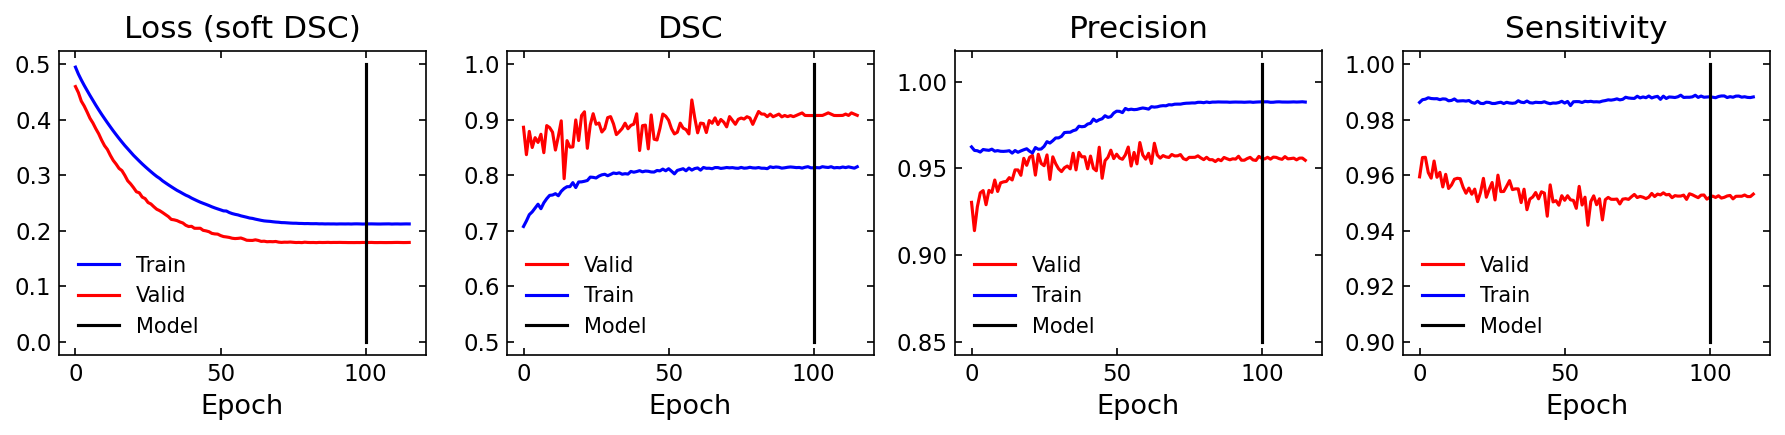
\includegraphics[width=\textwidth]{images/vacbag_metrics}
%     \caption{Model training metrics for canine imaging via soft DSC loss. \textbf{Final model selected at epoch 100} due to validation loss plateau. Training time 6 hours.}
%   \end{figure}
% \end{frame}
%
% ---------------------------- FRAME ---------------------------------
\begin{frame}{Canine imaging - Vacuum bag}
\begin{figure}
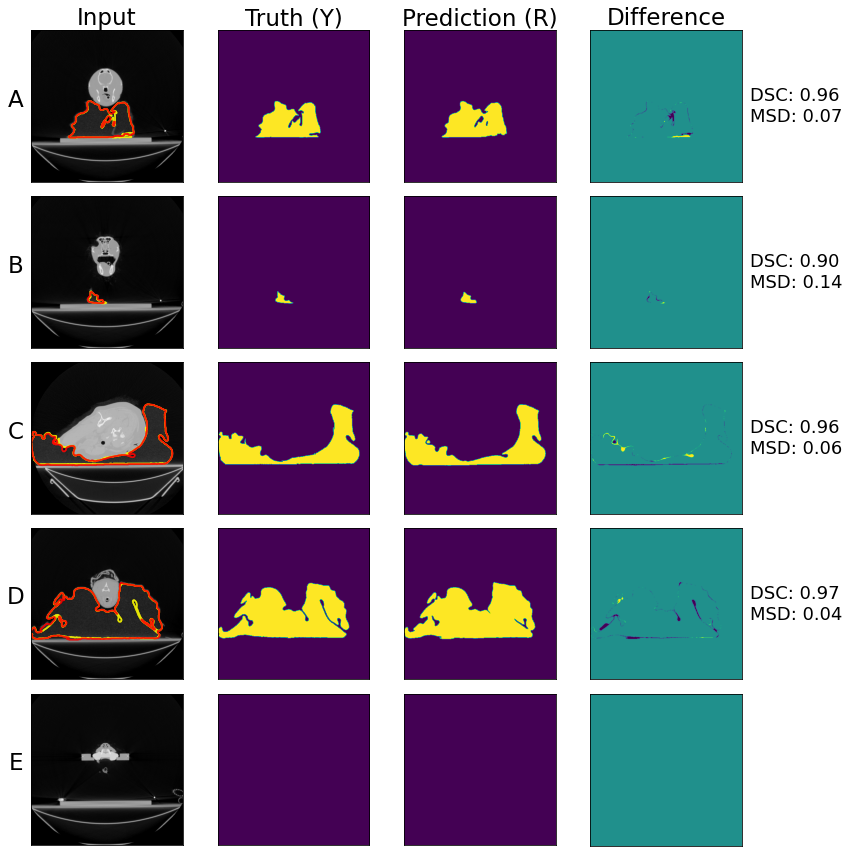
\includegraphics[width=0.665\textwidth]{images/vet_vacbag}
% \caption{Representative output for \textbf{vacuum bag}. Truth contour (yellow), prediction contour (red). Mean surface distance (MSD) mm.}
\end{figure}
\end{frame}
%
% ---------------------------- FRAME ---------------------------------
\section{Discussion}
\begin{frame}{Structure averaged metrics}
\begin{table}[h]
\footnotesize
\caption{Organ specific evaluation for proposed models on independent test dataset}
\centering
\begin{tabular}{c c c c c c}
              & sDSC  & DSC         & MSD (mm)  & Sensitivity & Specificity \\
\hline
\textbf{Pelvic imaging}      &              &              &              &       &       \\
Patient                      &              & 0.998(0.001) & 0.002(0.005) & 0.99 & 0.99 \\
Bladder ($\tau$ 1.46 mm)     & 0.9(0.2)     & 0.9(0.2)     & 1(3)         & 0.79 & 0.99 \\
Rectum ($\tau$ 6.99 mm)      & 0.9(0.1)     & 0.7(0.1)     & 1(2)         & 0.62 & 0.99 \\
Average                      &              & 0.9(0.2)     & 0.6(2)       & 0.99 & 0.99 \\ \\
\textbf{Canine imaging}      &              &              &              &       &       \\
Vacbag                       &              & 0.952(0.001) & 0.2(0.3)     & 0.95 & 0.99\\
\hline
\end{tabular}
\label{table:organ}
\end{table}


\vspace{4mm}
% \begin{itemize}
% \item Organ specific tolerance $\tau$ = MSD$_{95}$ (ie. Top 95\% expert performance).\footnotemark[3]
% \end{itemize}

\vspace{4mm}
\textbf{Cf. Expert IOV.}\footnotemark[2]
\begin{itemize}
\item Clinically 'acceptable' bladder and rectum DSC $\geq$ 0.7
% \item 'Excellent agreement' observed for expert rectum and bladder contours.
\item Bladder:  DSC 0.93 $\pm$ 0.03, MSD 0.9(0.3) mm.
\item Rectum:  DSC 0.81 $\pm$ 0.07, MSD 3(2) mm.
  % \item Organ specific tolerance $\tau$ = MSD$_{95}$ (ie. Top 95\% expert performance).\footnotemark[3]
\end{itemize}
\footnotetext[2]{\fullcite{Roach_2019}}
\footnotetext[3]{\fullcite{Nikolov_2018}}
\end{frame}
%
%\begin{frame}{Discussion: Structure specific metrics}
%\begin{table}[h]
\footnotesize
\caption{Organ specific evaluation for proposed models on independent test dataset}
\centering
\begin{tabular}{c c c c c c}
              & sDSC  & DSC         & MSD (mm)  & Sensitivity & Specificity \\
\hline
\textbf{Pelvic imaging}      &              &              &              &       &       \\
Patient                      &              & 0.998(0.001) & 0.002(0.005) & 0.99 & 0.99 \\
Bladder ($\tau$ 1.46 mm)     & 0.9(0.2)     & 0.9(0.2)     & 1(3)         & 0.79 & 0.99 \\
Rectum ($\tau$ 6.99 mm)      & 0.9(0.1)     & 0.7(0.1)     & 1(2)         & 0.62 & 0.99 \\
Average                      &              & 0.9(0.2)     & 0.6(2)       & 0.99 & 0.99 \\ \\
\textbf{Canine imaging}      &              &              &              &       &       \\
Vacbag                       &              & 0.952(0.001) & 0.2(0.3)     & 0.95 & 0.99\\
\hline
\end{tabular}
\label{table:organ}
\end{table}

%\textbf{Cf. S.O.T.A (TODO)}
%\begin{itemize}
%\item Small organ size $\downarrow$ performance.
%\end{itemize}
%\end{frame}
%

% ---------------------------- FRAME ---------------------------------
\section{Summary}
\begin{frame}{Conclusion and future work}
\textbf{Pelvic imaging model:}
\begin{itemize}
	\item Patient contouring within tolerances
	\item Suspect more data will improve bladder and rectum segmentation.
	\item 3D architecture may identify gaseous rectal volumes.
	 % - cf. S.O.T.A commercial DL solution (0.97, 0.79).\footnotemark[15]

	% S.O.T.A open-source DL solution (0.95, 0.92).\footnotemark[16]
	% \item Majority of surface correctly defined within tolerances for bladder and rectum
	% (sDSC 0.876, 0.922).
	% \item Weighted DSC loss significantly improved performance on class imbalanced data.
  \end{itemize}
  \vspace{4mm}

 \textbf{Canine imaging model:}
 \begin{itemize}
  \item Successfully deployed to clinic under a prototype warning
  \item Performance improvement of approximately 30 minutes per patient
\end{itemize}
% \footnotetext[15]{\fullcite{Wong2020}}
% \footnotetext[16]{\fullcite{Kazemifar_2018}}
\vspace{4mm}

\textbf{Future}
\begin{itemize}
\item Develop a soft surrogate for sDSC to optimise directly
\item U-Net no longer S.O.T.A $\implies$ HR-Net.\footnotemark[16]
\end{itemize}
\footnotetext[16]{\fullcite{Wang2020Deep}}
\end{frame}
%
% ---------------------------- FRAME ---------------------------------
% \begin{frame}{Conclusion: Future work}
% \textbf{Post-project goals:}
% \begin{itemize}
% \item Need for more data - limited dataset reduces generalisability.\footnotemark[17]
% \begin{itemize}
% \item S.O.T.A open-source: 600 - 1000 patients cf. 15.\footnotemark[3]
% \end{itemize}
% % \item Implement model at SASH for automatic vacuum bag contouring
% % \item Quantify use of sDSC as metric for clinical acceptability
% \item sDSC is a 'hard' metric. Developing a soft surrogate may allow for the direct optimisation of this metric
% \item Potential improvements under more complicated architecture


% \begin{itemize}
% \item Limited by cost and privacy constraints - minor improvement shown.\footnotemark[6]
% \end{itemize}

%ie. Downsampling layers.\footnotemark[17]
%\begin{itemize}
%	\item $\uparrow$ Learning of high level image feature
%	\item $\downarrow$ Resolution $\implies$ Harder to segment small organs
%\end {itemize}
% \end{itemize}
% \footnotetext[3]{\fullcite{Nikolov_2018}}
% \footnotetext[6]{\fullcite{Nemoto_2020}}
% \footnotetext[17]{\fullcite{Shen2017}}
%\footnotetext[17]{\fullcite{Zhu_2018}}
% \end{frame}


% ---------------------------- FRAME ---------------------------------

% \begin{frame}{Appendix sDSC cf. DSC}
% 	\begin{center}
% 		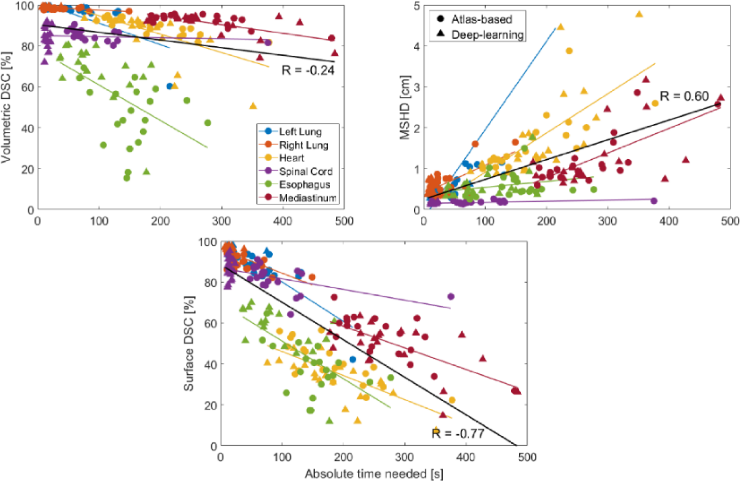
\includegraphics[width=0.80\textwidth]{images/vaassen}

% 		\caption{Comparison of common segmentation metrics with surface DSC (sDSC) for ability to infer absolute time required for automatic contour correction.\footnotemark[18]}
% 		\footnotetext[18]{\fullcite{Vaassen_2020}}
% 	\end{center}
% \end{frame}

% ---------------------------- FRAME ---------------------------------
\section{References}
\begin{frame}[t,allowframebreaks]{References} %% Aligned top
\printbibliography[heading=none]
\end{frame}

\end{document}
